\chapter{Experiment}
    This chapter describes about experimental setup in this study. The experiment is performed at Rare Isotope Beam Factory (RIBF) at RIKEN Nishina Center.\cite{RIKEN} A primary ${}^{48}$Ca beam is produced by the RIKEN accelerator complex and delivered to the BigRIPS separator. \cite{BigRIPS} The BigRIPS separator produced the ${}^{17}$B secondary beam which bombarded on the lead and carbon targets in front of the SAMURAI (Superconducting Analyzer for MUlti-particles from Radioisotope beams) spectrometer. \cite{SAMURAI} After the reaction at target, the fragments ${}^{15}$B and two neutrons are detected by detectors at SAMURAI area. Note that this experiment was part of the SAMURAI Dayone experiment which was the first physics run using the SAMURAI spectrometer.

\section{BigRIPS separator}

    \begin{figure}
        \centering
        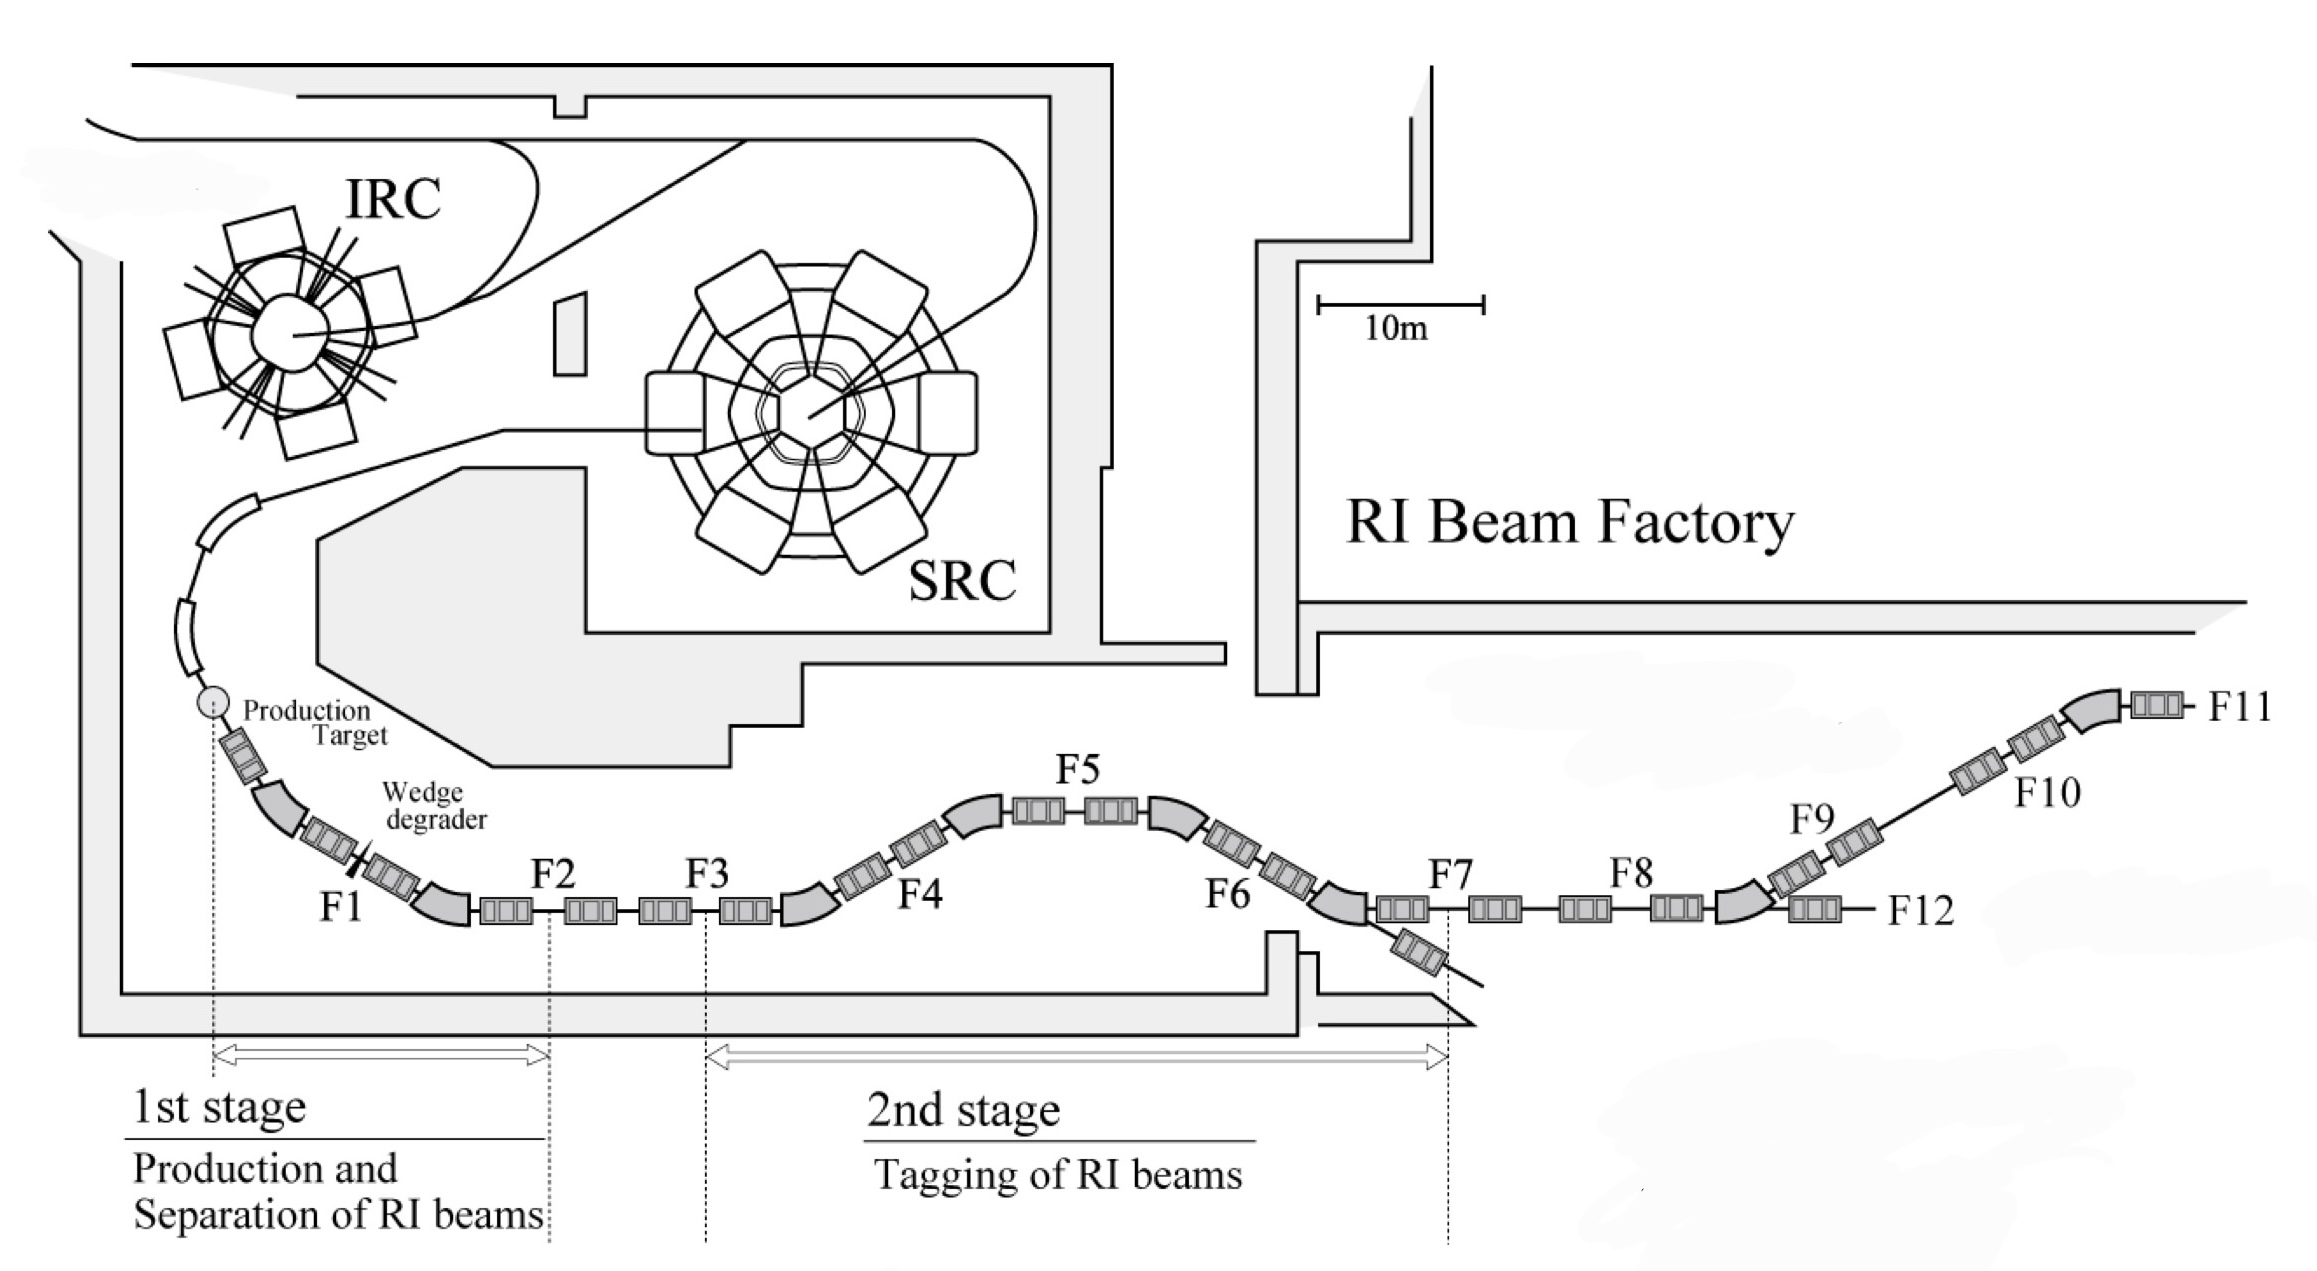
\includegraphics[width=12cm]{chapter3/BigRIPS_roof.jpg}
        \caption{A top view of the BigRIPS separator}
    \end{figure} 

After primary ${}^{48}$Ca beam is produced at SRC accelerator, the beam bombarded on a 30mm thick Be target and the secondary beam is produced through the in-flight fragmentation method. Since the secondary beam includes many rare isotopes, the RI beam is separated by the BigRIPS separator. Table 3.1 shows the BigRIPS separator setup for Dayone experiment. In the first stage of BigRIPS separator, the RI beam separated by dipole magnet with slit and wedge-shaped degrader located at F1 focal plane. In the dipole magnet, the rigidity of a particle can be written as following eq. 3.1
    \begin{align}
        \rho = \frac{A}{Z} \cdot\frac{v}{B}
    \end{align}
The velocity of the secondary beam is almost same regardless of the nuclei so that it can be possible to choose specific $A/Z$ by adjusting the slit to filter only some $B\rho$ value. After that, the wedge-shaped degrader makes the beam energy depends on the $Z$ so that even same $A/Z$ nuclei can be separated. In the second stage, the RI beam is identified using TOF-B$\rho$-$\Delta E$ method. Each detector information will be described as following.
    \begin{table}[h]
        \centering
        \begin{tabular}{c c c c}
            \hline
            Focal Plane & Dipole Magnet [Tm] & Slit[mm] & Degrader / Detector \\
            \hline
            F0  & 9.1734 &  & Be target (30mm) \\
            F1  & 8.8195 & $\pm$120 & Al wedge degrader \\
            F2  & 8.8195 & L: 10 R: 7 & \\
            F3  & 8.7841 &  & Plastic Scintillator (3mm)\\
            F5  & 8.780  & $\pm$120 & BPC \\
            F7  & 8.780  & $\pm$120 & Plastic Scintillator (3mm)\\
            %F13 &  & & Plastic Scintillator (0.5mm$\times$2)\\
            \hline
        \end{tabular}
        \caption{BigRIPS separator setup for Dayone experiment \cite{Dayonelog}}
    \end{table}

\subsection{Plastic Scintillator}
At focal plane F3, F7, F13, plastic scintillators are located for measuring the time of flight (TOF) of secondary beam. In F3 and F7, plastic scintillator with 3mm thickness is located and at F13 there are two scintillators, SBT1 and SBT2, with 0.5mm thickness. The flight length between F7 and F13 (Average point of SBTs) is .

\begin{table}[h]
    \centering
    \begin{tabular}{c|ccc}
        \hline
        & Location & Thickness & Distance from target upstream \\
        \hline
        SF3 & F3 & 3mm & \\
        SF7 & F7 & 3mm & \\
        SBT1 & F13 &0.5mm & \\
        SBT2 & F13 &0.5mm & \\
        \hline
    \end{tabular}
    \caption{Plastic Scintillators at F3, F7, F13}
\end{table}


\subsection{BPC (Beam Proportional Chamber)}
BPC is Multi Wire Proportional Chamber (MWPC) located at F5 focal plane which is used for measuring the position of beam. The purpose of BPC is tagging magnetic Rigidity of secondary beam.
\begin{table}[h]
    \centering
    \begin{tabular}{l|c}
        \hline
        Effective Area & (H)240mm x (V)150mm \\
        Configuration & $XX$ (2 Planes) \\
        number of wire & 64 $\times$ 2 = 128 \\
        Wire Pitch & 4mm \\
        Gas & $i$--${C}_{4} {H}_{10}$ at 50 torr\\
        \hline
    \end{tabular}
    \caption{Parameter of BPC (Beam Proportional Chamber)}
\end{table}

\clearpage

\begin{figure}[h]
    \centering
    \begin{subfigure}[h]{\textwidth}
        \centering
        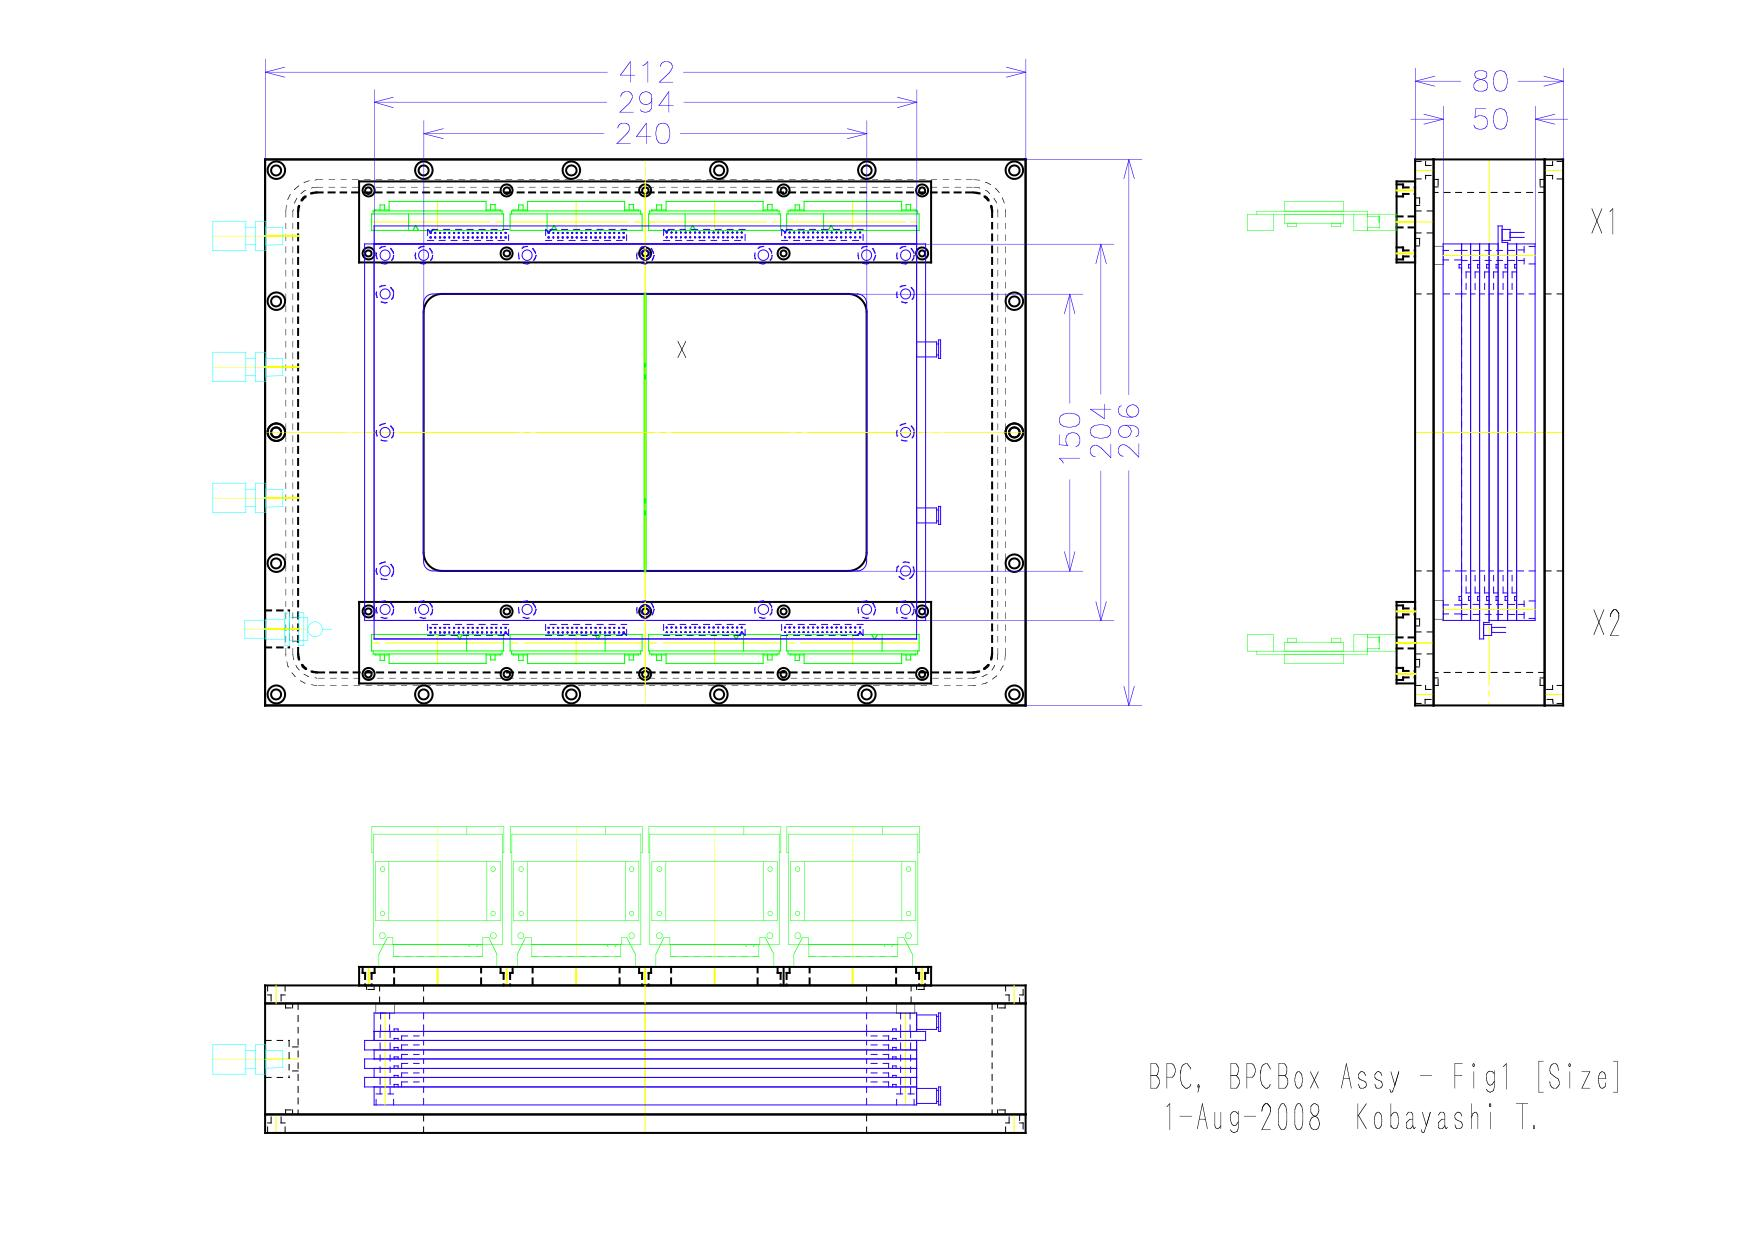
\includegraphics[width=12cm]{chapter3/bpc_a1.jpg}
    \end{subfigure}
    \begin{subfigure}[h]{\textwidth}
        \hspace{2.4cm}
        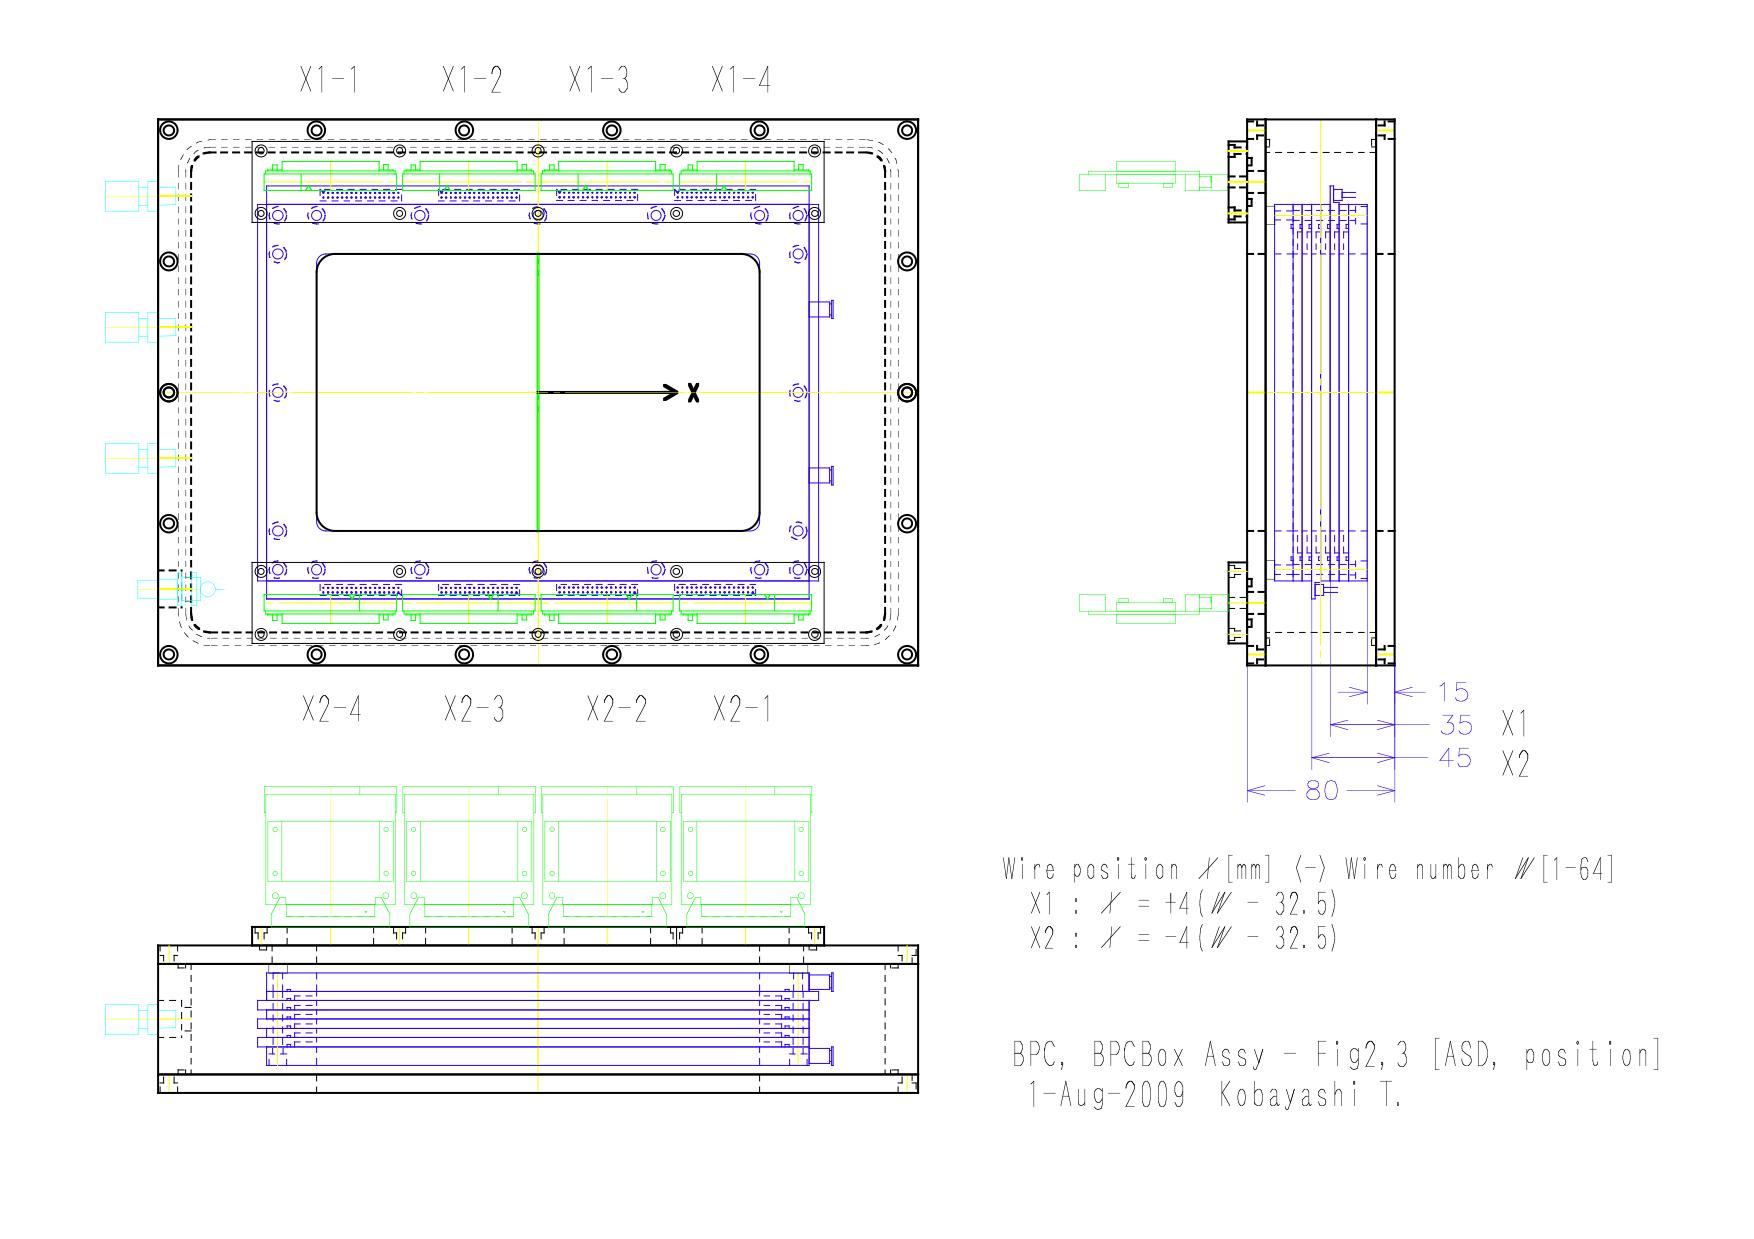
\includegraphics[width=12.5cm]{chapter3/bpc_a23.jpg}
    \end{subfigure}
        \caption{BPC (Beam Proportional Chamber) Assembly}
\end{figure}

\subsection{ICB (Ion Chamber for Beam)}
The ICB is ionization chamber for measuring the energy loss ($\Delta E$) of secondary beam.
\begin{table}[h]
    \centering
    \begin{tabular}{l|c}
        \hline
        Effective Area & (H)140mm x (V)140mm x (D)420mm\\
        Configuration & 10 anodes and 11 cathodes \\
        Anode-cathode gap & 21mm \\
        Gas & P10 at 1 atm\\
        Distance from target upstream & ??m \\
        \hline
    \end{tabular}
\end{table}

\begin{figure}[t]
    \centering
    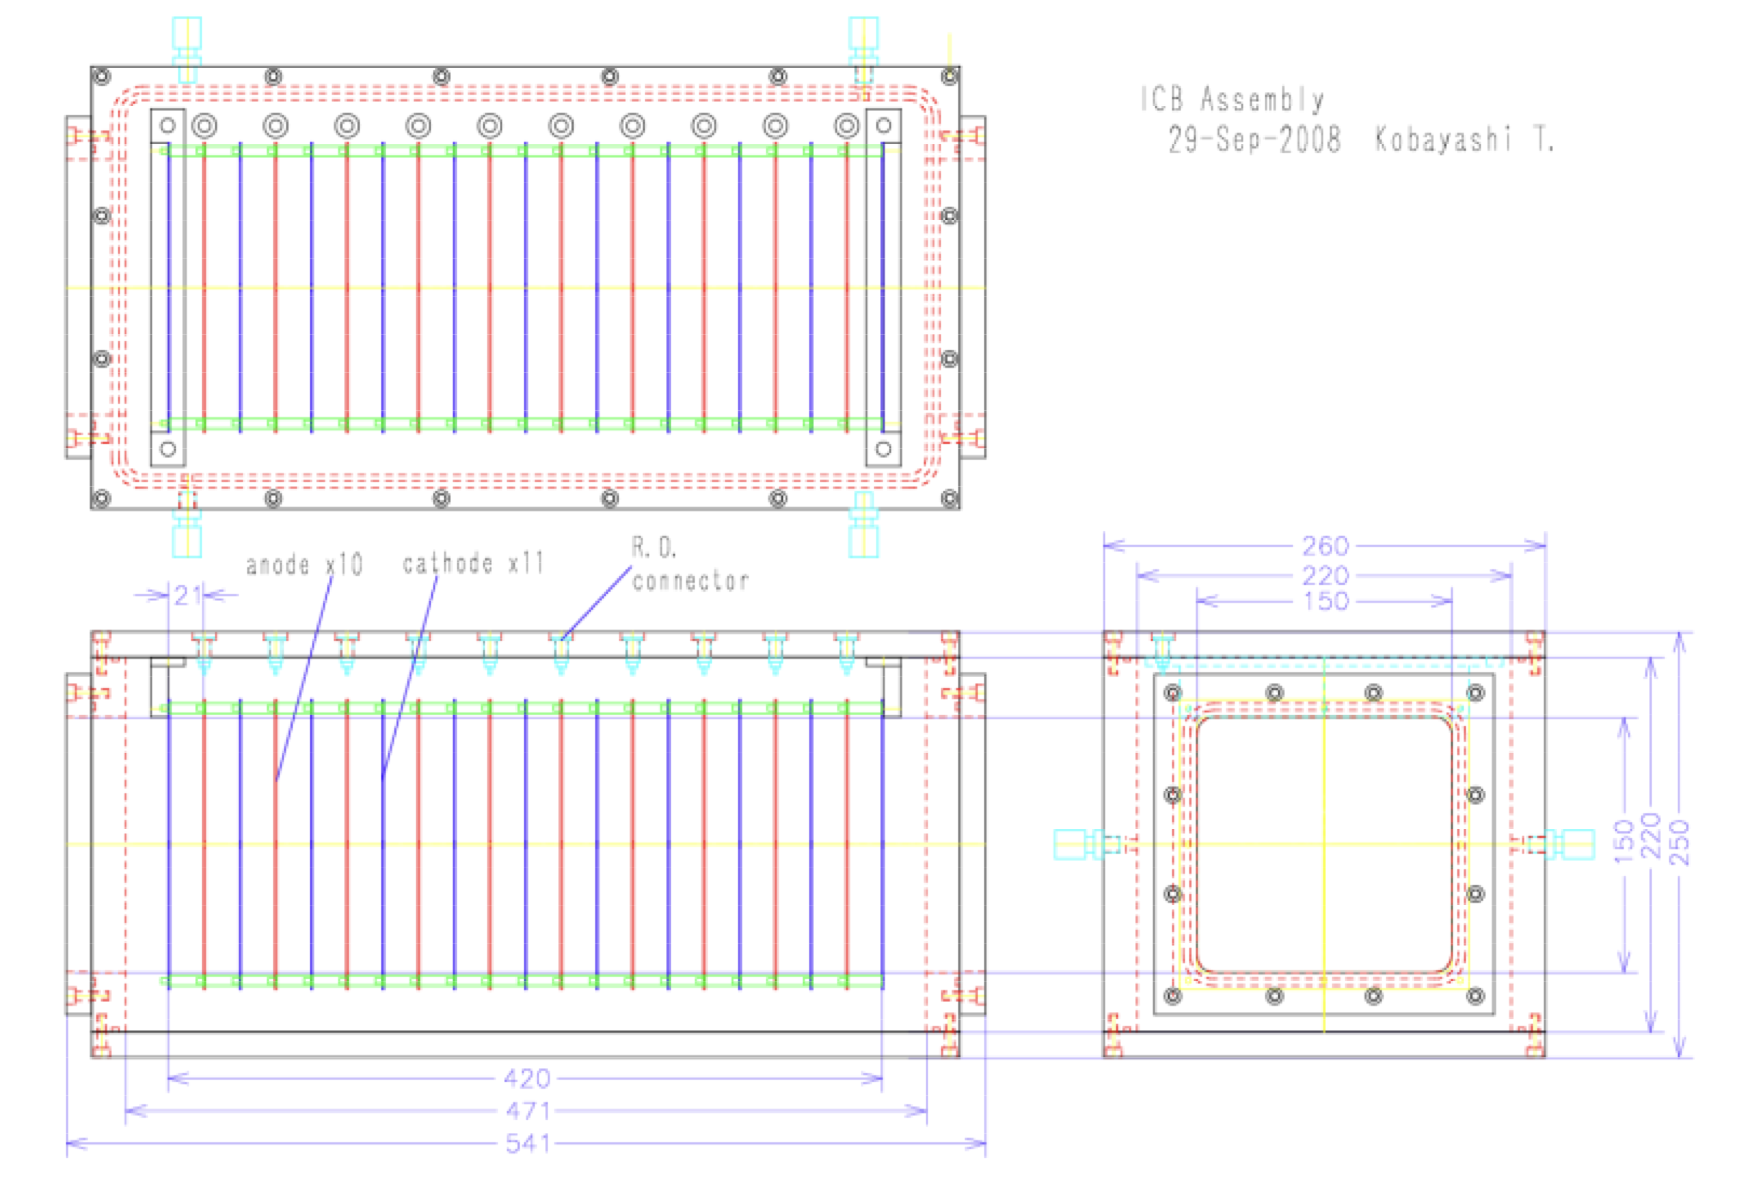
\includegraphics[width=12cm]{chapter3/icb_a}
    \caption{ICB (Ion Chamber for Beam) Assembly}
\end{figure}

\subsection{BDC1, BDC2 (Beam Drift Chamber)}
There are two Beam drift chamber for reconstructing the trajectory of secondary beam. 

\begin{table}[h]
    \centering
    \begin{tabular}{l|c}
        \hline
        Effective Area & (H)80mm x (V)80mm\\
        Configuration & $XX'YY'XX'YY'$ (8 planes)\\
        Number of Wire & 16 $\times$ 8 = 128 \\
        Wire Pitch & 5mm \\
        Gas & $i$--${C}_{4} {H}_{10}$ at 100 torr\\
        Distance from target upstream & ??m \\
        \hline
    \end{tabular}
\end{table}

\begin{figure}[h]
    \centering
    \begin{subfigure}{\textwidth}
        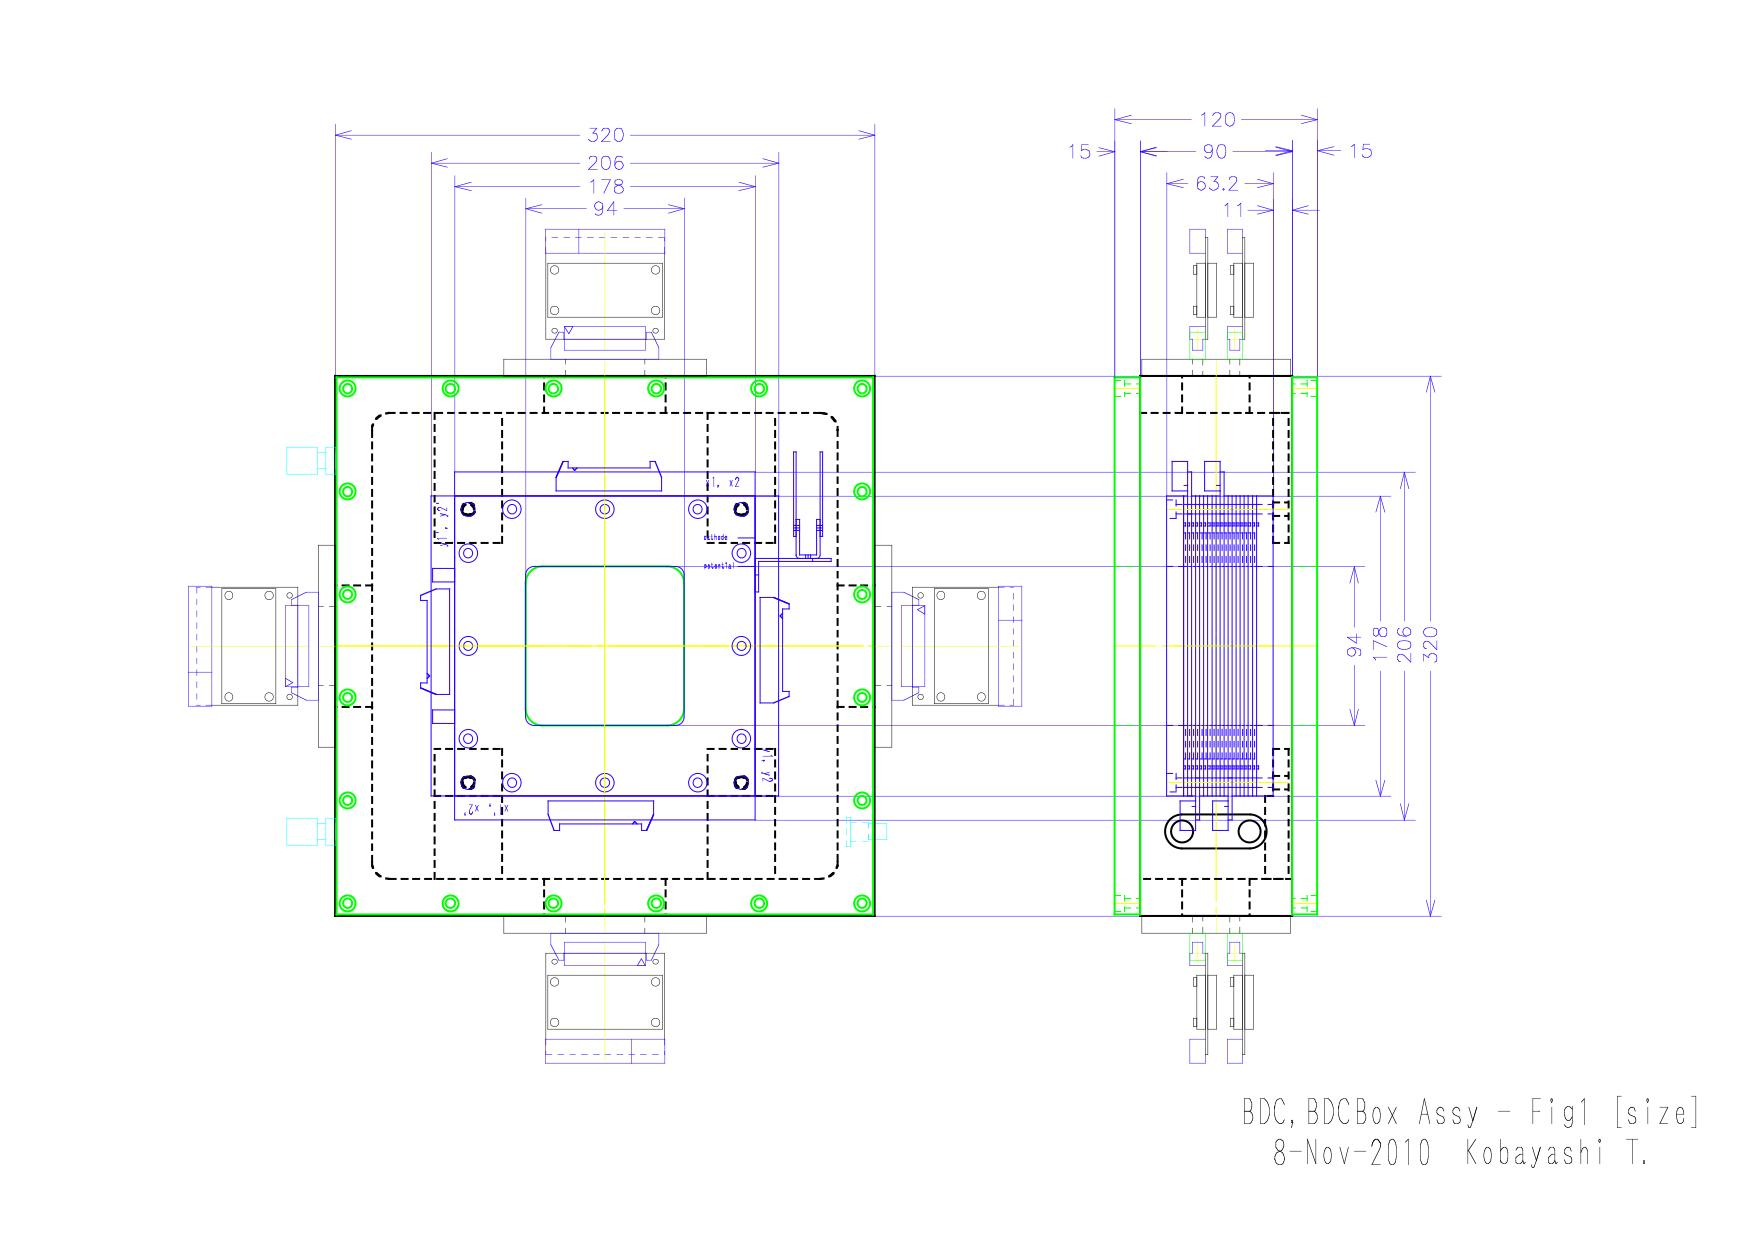
\includegraphics[width=12cm]{chapter3/bdc_a1.jpg}    
    \end{subfigure}
    \begin{subfigure}{\textwidth}
        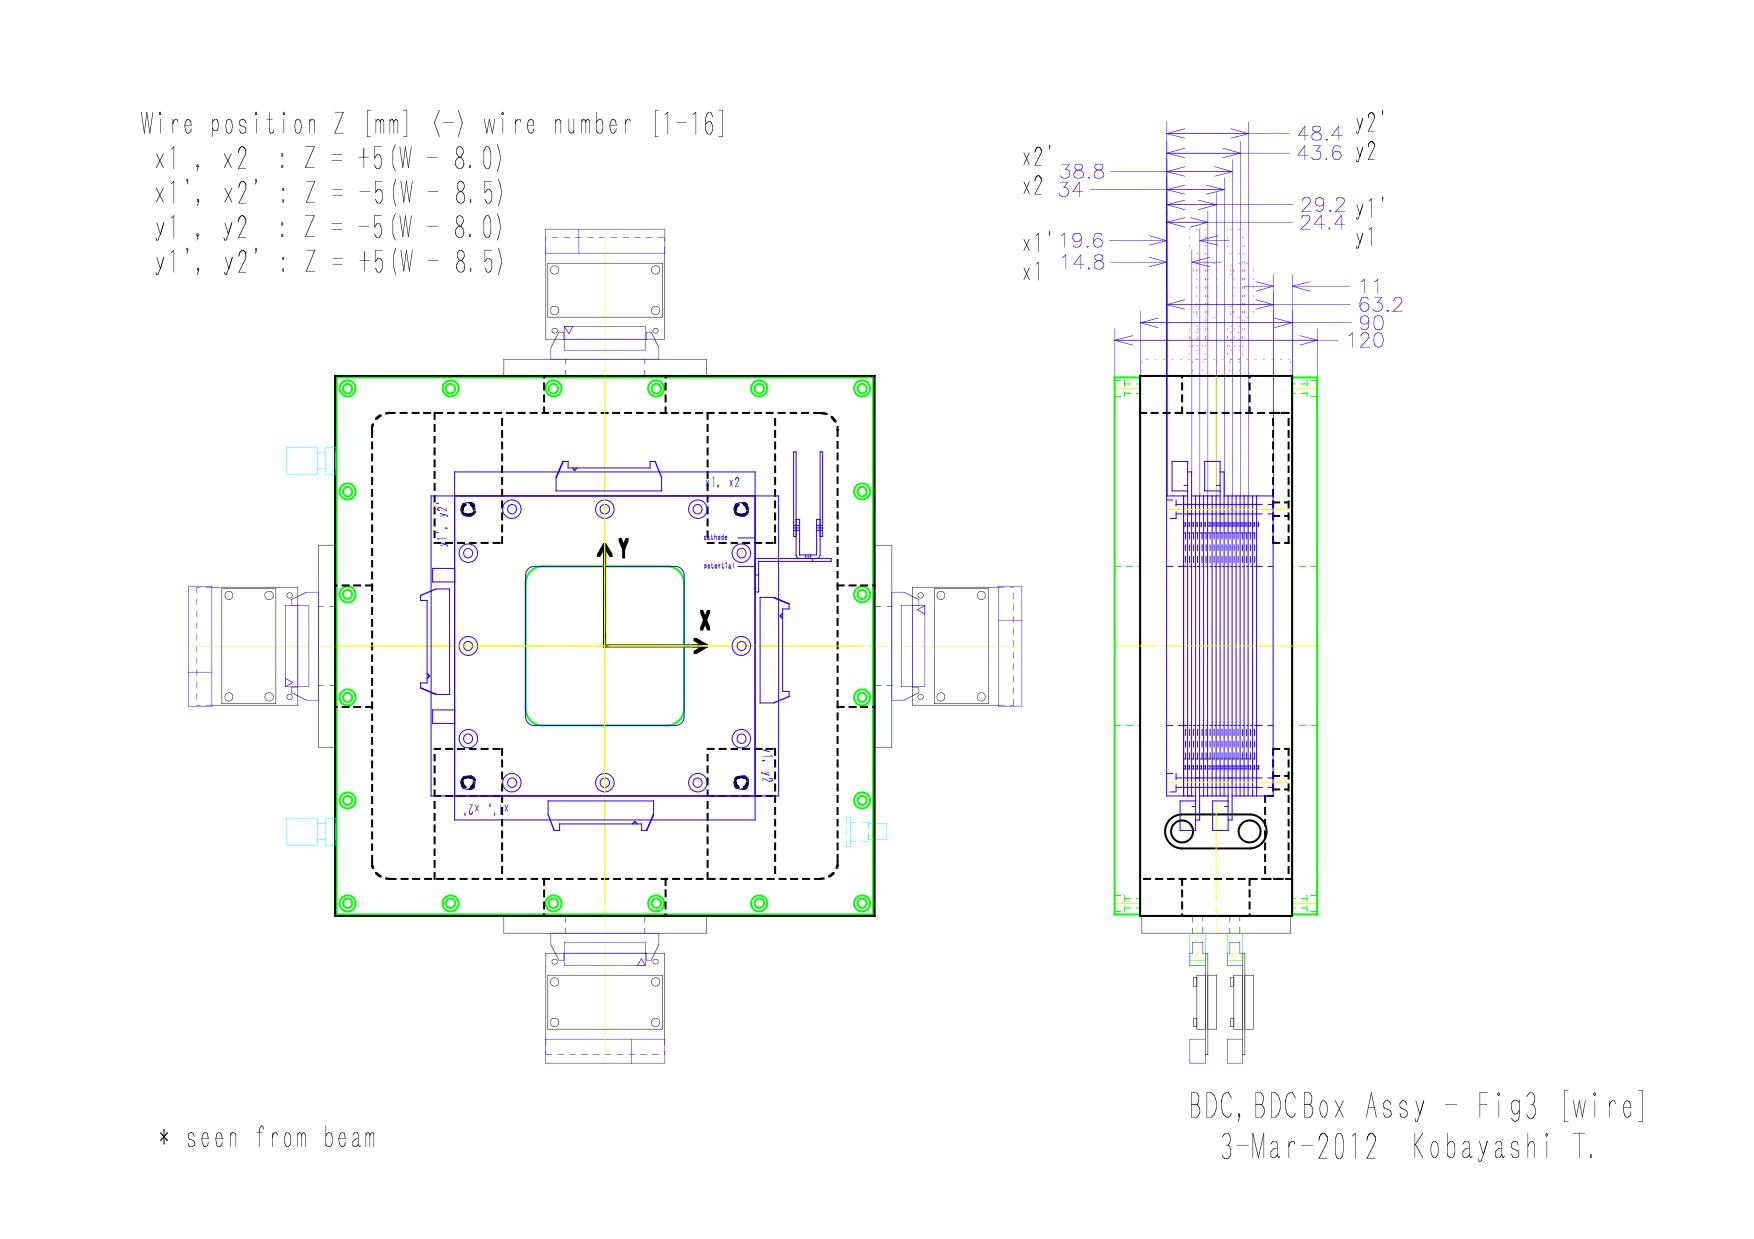
\includegraphics[width=12cm]{chapter3/bdc_a3.jpg}
    \end{subfigure}
    \caption{BDC (Beam Drift Chamber) Assembly}
\end{figure}

\section{SAMURAI}
The SAMURAI spectrometer is designed for kinematically complete experiment such as invariant mass spectroscopy. \cite{SAMURAIConcept} 
\subsection{SAMURAI Magnet}

\subsection{FDC1, FDC2 (Forward Drift Chamber)}
\begin{table}[h]
    \centering
    \begin{tabular}{l|c}
        \hline
        Effective Area & (H)400mm x (V)300mm x (D)180mm\\
        Configuration & $XX'UU'VV'XX'UU'VV'XX'$ (14 planes)\\
        Number of Wire & 32 $\times$ 14 = 448 \\
        Wire Pitch & 10mm \\
        Gas & $i$--${C}_{4} {H}_{10}$ at 50 torr\\
        Distance from target upstream & ??m \\
        \hline
    \end{tabular}
    \caption{Parameter of FDC1}
\end{table}
\begin{table}[h]
    \centering
    \begin{tabular}{l|c}
        \hline
        Effective Area & (H)2296mm x (V)836mm x (D)860mm\\
        Configuration & $XX'UU'VV'XX'UU'VV'XX'$ (14 planes)\\
        Number of Wire & 112 $\times$ 14 = 1568 \\
        Wire Pitch & 20mm \\
        Gas & He + 50\% ${C}_{2} {H}_{6}$ at 1 atm\\
        \hline
    \end{tabular}
    \caption{Parameter of FDC2}
\end{table}
\subsection{HODF (HODoscope for Fragment)}
\begin{table}[h]
    \centering
    \begin{tabular}{l|c}
        \hline
        Effective Area & (H)1600mm x (V)1200mm x (D)10mm\\
        Number of Scintillator & 16 \\
        Width of Scintillator & 10mm \\
        \hline
    \end{tabular}
    \caption{Parameter of HODF}
\end{table}

\subsection{NEBULA}
For measuring momentum vector of neutron, 

\section{Electronics}
\subsection{Trigger and Livetime}
There are four triggers condition which are used in this experiment; DSB, B$\times$N, B$\times$N, B$\times$N. They are defined as follows.
\begin{enumerate}
    \item \textbf{DBS} (Down Scale Beam) 
    \item \textbf{B$\times$N} (Coincidence between Beam and NEBULA)
    \item \textbf{B$\times$D} (Coincidence between Beam and DALI)
    \item \textbf{B$\times$H} (Coincidence between Beam and HODF)
\end{enumerate} 
\subsection{}
\section{Run summary}
\begin{center}
    \begin{tabular}[h]{ccc}
         hline
        Run number& Target & Trigger \\
        394 - 404 &  C (1.8 g/cm${}^{2}$)  & DSB(1/20) + B x N + D(1/1)\\
        405 - 409 &  Empty  & DSB(1/20) + B x N + D(1/1)\\
        410 - 427 &  Pb (3.0 g/cm${}^{2}$)  & DSB(1/20) + B x N + D(1/1)\\
        428 - 431 & Pb (3.0 g/cm${}^{2}$)  & DSB(1/20) + B x N + D(1/1)\\
    \end{tabular}
\end{center}

\section{Material between F7 to target}
\section{Secondary Target}
본 실험의 19B런에서는 카본 타겟과 납 타겟을 사용하였다. 카본 타겟의 두께는 10mm, 납 타겟의 두께는 1mm의 것과 2mm의 것을 겹쳐서 사용하였다. 